\documentclass[a4paper,10pt,twocolumn]{article}
%\usepackage{xeCJK}
%\setCJKmainfont{SimSun}
\usepackage{CJKutf8}
\usepackage{cite}
\usepackage{listings}
\usepackage[T1]{fontenc}
\usepackage{amsmath}
\usepackage{amssymb}
\usepackage{graphicx}
\usepackage[]{circuitikz}
\setlength{\oddsidemargin}{0in}
\setlength{\topmargin}{-.8in}
\setlength{\textheight}{9.7in} \setlength{\textwidth}{6.5in}
\usepackage{color,hyperref}
\definecolor{darkblue}{rgb}{0.0,0.0,0.3}
\hypersetup{colorlinks,breaklinks,
            linkcolor=darkblue,urlcolor=darkblue,
            anchorcolor=darkblue,citecolor=darkblue}
\providecommand*\url[1]{\href{#1}{#1}}
\renewcommand*\url[1]{\href{#1}{\texttt{#1}}}

\newcommand{\bm}[1]{\boldsymbol{#1}}
\newcommand{\bh}[1]{\boldsymbol{\hat{#1}}}
\newcommand{\bt}[1]{\boldsymbol{\tilde{#1}}}
\newcommand{\bbar}[1]{\boldsymbol{\bar{#1}}}
\newcommand{\mbf}[1]{\ensuremath{\mathbf{#1}}}
\newcommand{\ode}[2]{\ensuremath{\frac{\mathrm{d} #1}{\mathrm{d} #2}}}
\newcommand{\odet}[2]{\ensuremath{\tfrac{\mathrm{d} #1}{\mathrm{d} #2}}}
\newcommand{\oden}[3]{\ensuremath{\frac{\mathrm{d}^#3 #1}{\mathrm{d} #2^#3}}}
\newcommand{\pde}[2]{\ensuremath{\frac{\partial #1}{\partial #2}}}
\newcommand{\pdet}[2]{\ensuremath{\tfrac{\partial #1}{\partial #2}}}
\newcommand{\pden}[3]{\ensuremath{\frac{\partial^{#3} #1}{\partial
      #2^{#3}}}}
\newcommand{\sub}[1]{\ensuremath{_{\rm{#1}}}}
\newcommand{\arriba}[1]{\ensuremath{^{\rm{#1}}}}
%
\newcommand{\N}{\ensuremath{\mathbb{N}}}
\newcommand{\R}{\ensuremath{\mathbb{R}}}
\newcommand{\C}{\ensuremath{\mathbb{C}}}
\newcommand{\ee}[1]{\ensuremath{\mathrm{e}^{#1}}}
\newcommand{\hdos}{\ensuremath{\mathrm{H}_2}}
\newcommand{\COdos}{\ensuremath{\mathrm{CO}_2}}
\newcommand{\ATP}{\ensuremath{\mathrm{ATP}}}

\newcommand{\dt}{\ensuremath{\mathrm{d}t}}
\newcommand{\dtau}{\ensuremath{\mathrm{d}\tau}}
\newcommand{\DV}{\ensuremath{\Delta V}}
\DeclareMathOperator{\Li}{\mathcal {L}^{-1}}
\DeclareMathOperator{\Lin}{\mathcal {L}^{-1}}
\DeclareMathOperator{\sinc}{\text{sinc}}
\DeclareMathOperator{\sign}{\mathrm{sign}}
\newtheorem{remark}{Remark}
%\usepackage[utf8x]{inputenc}
%%
\title{围棋 \\ The Game of Go\\ \small Modeling Complex Systems\\ DMKM}
\author{Carlos López Roa\\ \href{mailto:me@mr3m.me}{me@mr3m.me}}
\date{\today}
\pdfinfo{%
  /Title    ()
  /Author   (CLR)
  /Creator  ()
  /Producer ()
  /Subject  ()
  /Keywords ()
}
\begin{document}
\begin{CJK*}{UTF8}{gbsn}
\maketitle
%%% Content
\begin{abstract}
https://youtu.be/Wvm0ZgCsm1E
https://github.com/mr3m/GameOfGo
\end{abstract}

%\tableofcontents

\section{Introduction}
The game of Go, also known as {Wéiqí: 围棋} in Chinese, which means literally \emph{surround game}, is a two-player board game in which the aim is to surround more territory that the opponent \cite{Kunkle2002}.

It was originated in ancient China more than 2,500 years ago (figure \ref{l1}). It was considered one of the four essential arts\footnote{The four arts ({siyi: 四艺}): To play the guqin, a stringed instrument ({Qín:  琴}), the strategy game of Go ({Qí:  棋}), Chinese calligraphy ({Shu:  书}), Chinese painting ({Huà:  画}) } of a cultured Chinese scholar.

\begin{figure}[!ht]
\begin{center}
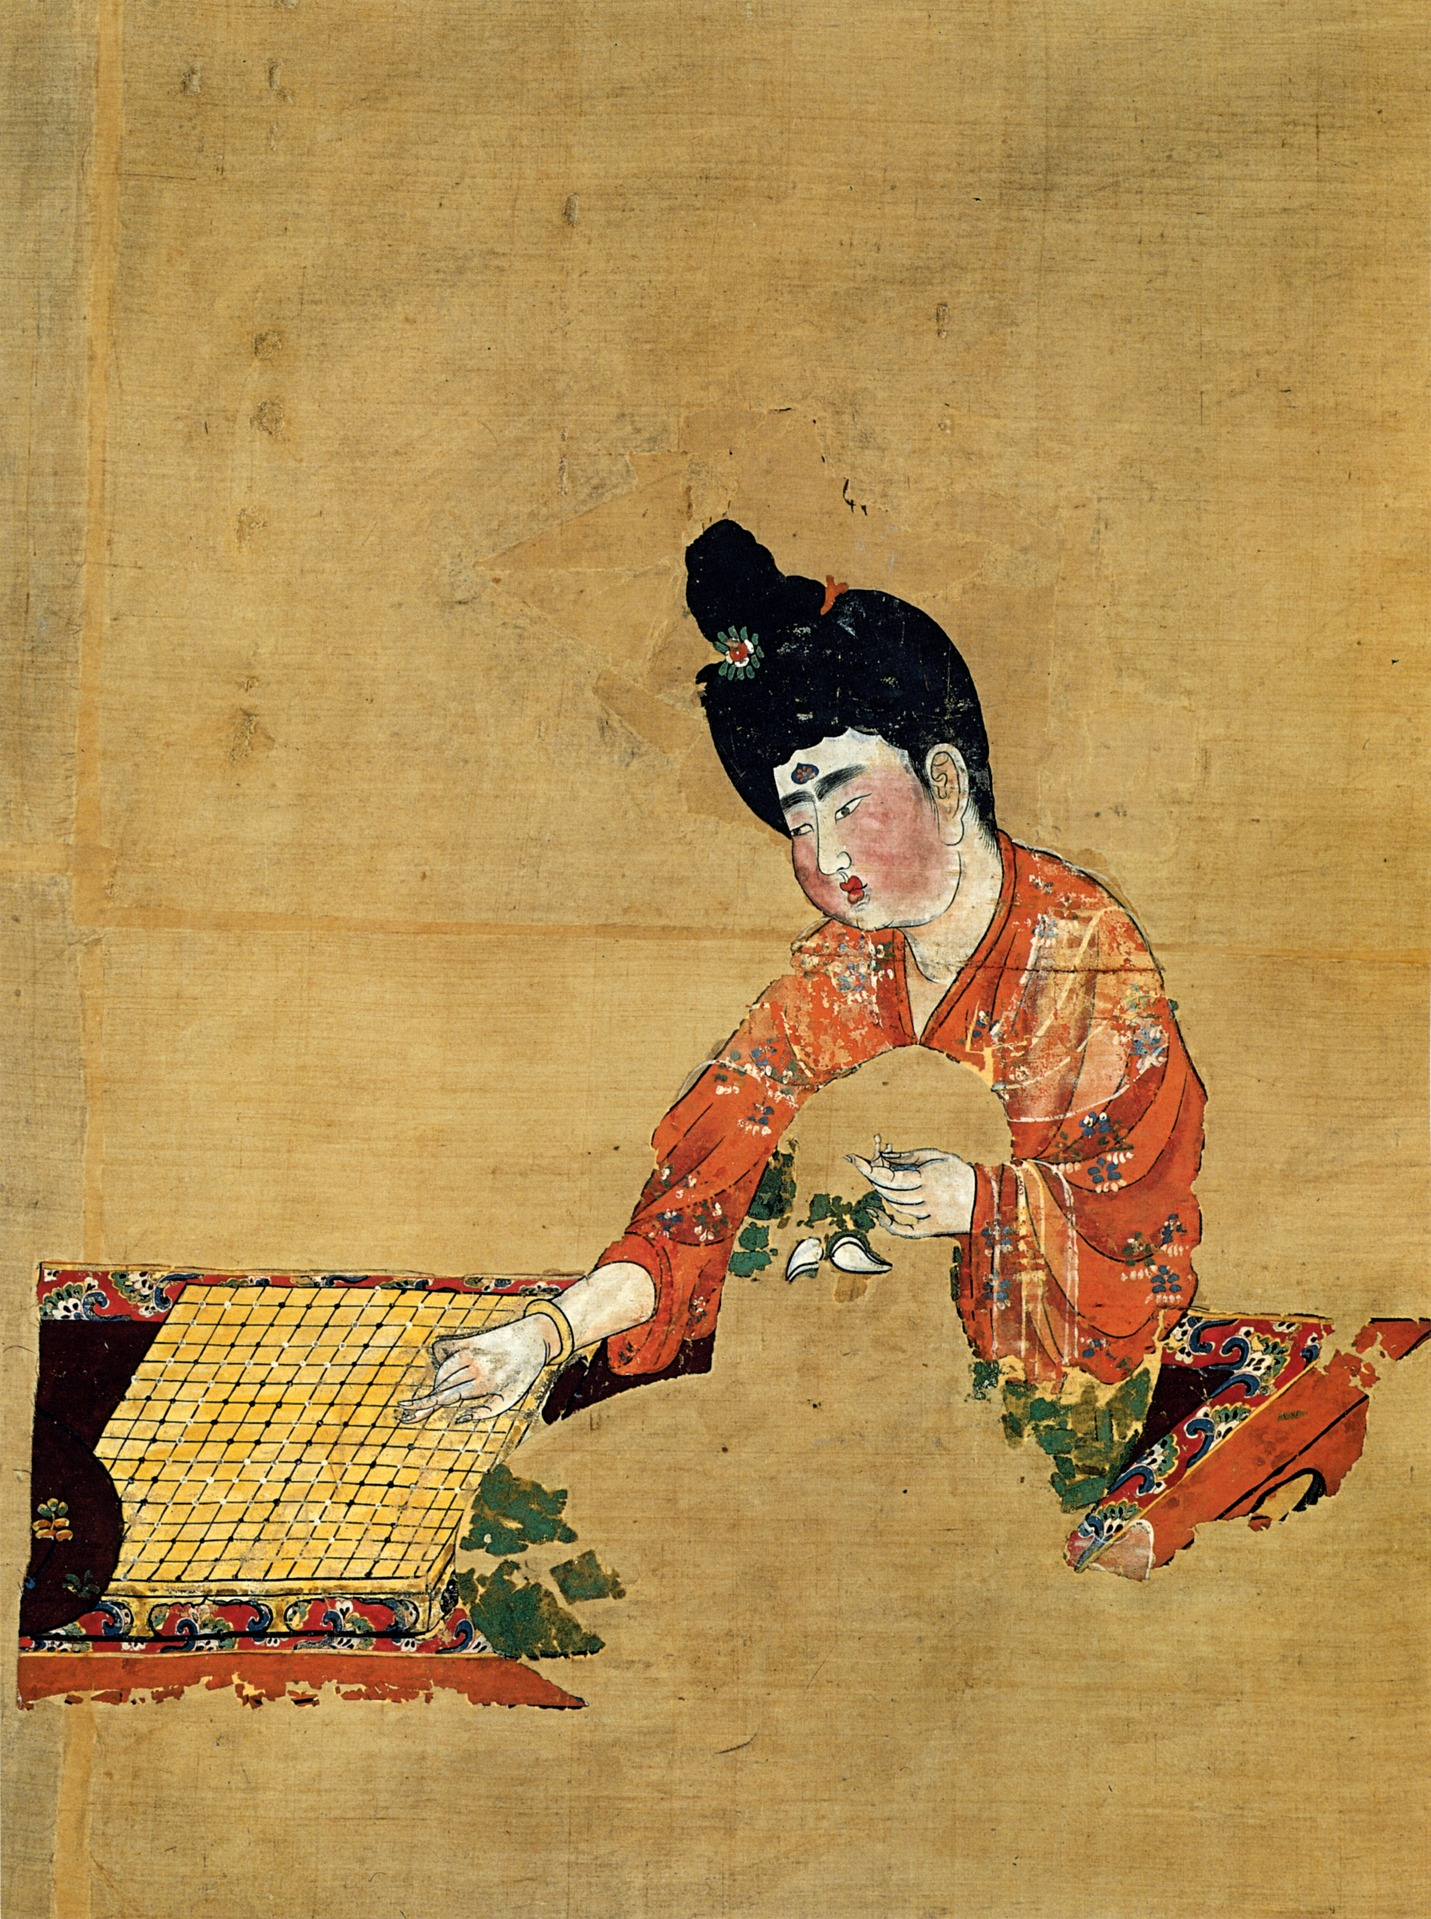
\includegraphics[width=4cm]{Astana.jpg}
\caption{\footnotesize{Woman Playing Go (Tang Dynasty c. 744), discovered at the Astana Graves}\label{l1}}
\end{center}
\end{figure}

Despite it's relative simple rules, the relative complexity of Go with respect to Western chess is far more superior ($10^{761}$ compared to $10^{120}$ possible games).

Precisely because of this great complexity is that, different from chess which was \emph{conquered} by IBM's \textsc{Deep blue} in 1996 agains't world's Grand Master \textsc{Gary Kaspárov}, no equivalent conquest has been achieved by computer go until recent victory of Google's \textsc{Alpha Go} agains't \textsc{Fan Hui} the European Go Champion \cite{Silver2016a}. 

In this study we took a multiagent system approach to the problem of computer Go, first, a description of the implementation is made, after some tests were carried out and described at the end some conclusions and future work are drawn.

%\subsection{State of the art}

\subsection{Game Mechanics}
The two players alternately place black and white playing pieces, called \emph{stones}, on the vacant places of a board with a 19×19 grid of lines. 

Each stone is said to have 4 \emph{liberties} ({Qì:  气})  when the four orthogonal-adjacent points are empty, this stone loses each of it's liberties whenever a stone is placed in this points. If the recently placed stone is of the opposite color, then the liberty is just lost, however, if the recently placed stone is of the same color, the individual liberty is lost and a \emph{group} liberty is created, composed of the sum of the liberties of these two stones. Generalizing the previous principle, one can form huge groups of stones of the same color, which have a collective liberty. The particular form of this groups is essential part of the strategy of the game. 

Once placed on the board, stones may not be moved, but stones may be removed from the board if captured. A stone (or group of stones) it's captured by the opponent when all the liberties are suppressed.

 An enclosed liberty (or liberties) is called an \emph{eye}\footnote{see figure \ref{f1}} (眼), and a group of stones with at least two separate eyes is said to be unconditionally \emph{alive}. Such groups cannot be captured, even if surrounded. \emph{Dead} stones are stones that are surrounded and in groups with poor shape (one or no eyes), and thus cannot resist eventual capture.

\begin{figure}[!ht]
\begin{center}
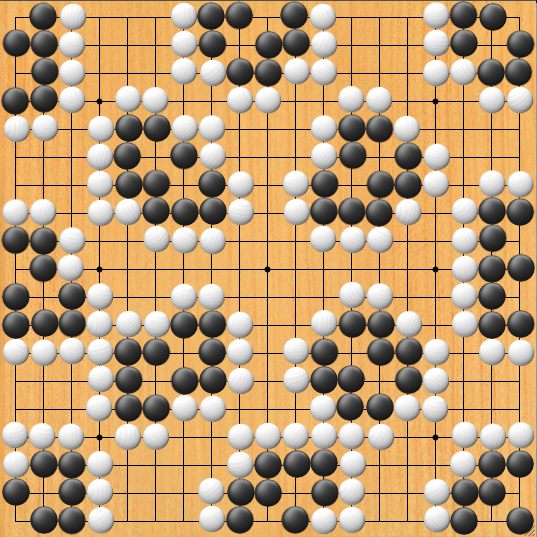
\includegraphics[width=5.5cm]{eyes.png}
\caption{\footnotesize All the smallest groups with two eyes by blacks, enclosed by whites without being able to capture the groups \label{f1}}
\end{center}
\end{figure}

There are only two rules in Go, namely: 

\begin{enumerate}
\item \textbf{The rule of Liberty}: Every stone remaining on the board must have at least one liberty.
\item \textbf{The ko rule (劫)}: The stones on the board must never repeat a previous position of stones
\end{enumerate}

Remark that by rule 1, suicide moves are forbidden, that is jumping into an eye of the opponent contained in a at-least-two-eye-group; if the group is a one-eye-group then this move is allowed. Also please note that to blocks one eye, though permitted is by no means desired, since it can turn alive groups into dead ones. Also as a common consensus, blacks play first.   

The two players place stones alternately until they reach a point at which neither player wishes to make another move. When a game concludes, the territory is counted along with captured stones to determine the winner. 

\section{Implementation}
A box world was set up in NetLogo, to represent the board game, that is, with no periodicity in the edges.  

In this world, two computers play Go agains't each other. Though, the computer players are composed of the collective decision of the stones placed in the board, that is, using the distributed artificial intelligence approach of multiagent systems. 

The stones were modeled using reactive agents, the environment is a 19x19 closed two dimensional grid, all agents share the same organization, the interaction between each other happens when they share a liberty. Also agents of the same color connected through their liberties form undirected links between each other.  The goal, is the same as the game, to occupy the most territory.  The game ends when both agent types pass consecutively. 

\subsection{Making a move}
A general overview of the game dynamics can be seen in the flow diagram \ref{d1}

\begin{figure}[!ht]
\begin{center}
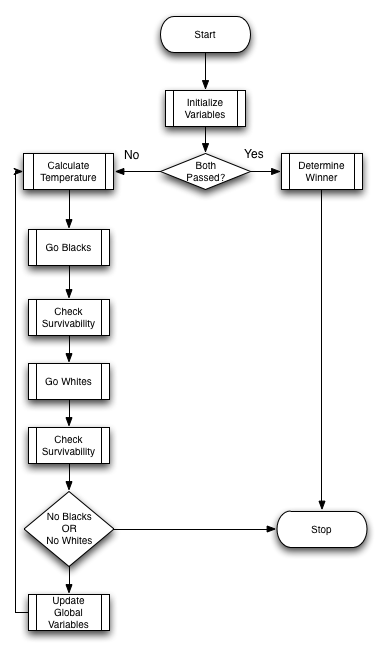
\includegraphics[width=7cm]{df.png}
\caption{\footnotesize {Flow diagram of the main components of the program.} First we initialize the variables. A if condition governs the flow, which is the condition to end the game.  \label{d1}}
\end{center}
\end{figure}

Each turtle has four internal variables: The number of liberties, the number of captured stones, the liberties of the group in which they are in, and a boolean variable related to the exploration of groups. 
 
Each patch in the environment has a temperature associated, which is composed of the number of stones surrounding this patch, that is a measure of liberty of the patch. 

To make a move, we follow the flow described in diagram \ref{d2}

\begin{figure}[!ht]
\begin{center}
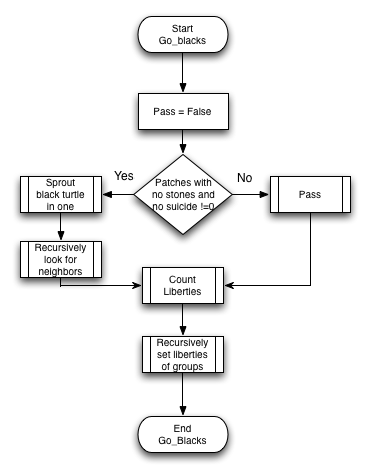
\includegraphics[width=7cm]{go_blacks.png}
\caption{\footnotesize Flow to play blacks. To play whites is simmetrical. A IF statement looks for free patches, if found a black turtles is sprout and related with it's neighbours recursively, if not then blacks pass. Then this stone is assigned their liberties, and the groups get the liberties recalculated.\label{d2}}
\end{center}
\end{figure}

To calculate the liberties of one turtles is just to subtract the number of stones in the neighboring spaces from the number of neighboring spaces\footnote{corner stones get between 3 and 2 instead of 4 neighboring spaces}, the group liberty is defined as the sum of the individual liberties. If both the individual liberty and the group one are equal to zero, then the stone (group) dies. 

The discovery of the group of one stones is done by asking each stone to name it's neighbors recursively, when all neighbors have been named, then we assign an undirected link between this stone and all the named neighbors. This due to the transitivity: If $A$ is neighbor of $B$ and $B$ is neighbor of $C$ then $A$ is neighbor of $C$.

Thing to note, is that because of the condition to pass, then it's not possible to commit suicide or to block owns eyes. 

\section{Results}

\section{Conclusions}

\section{Future Work}



\bibliography{/Users/Poincare/Dropbox/Tex/library.bib}
\bibliographystyle{siam}
\end{CJK*}
\end{document}